\chapter{Des solutions légères de \emph{machine learning} pour les archives}

\subsection{\gls{TAL} pour la classification~: \emph{clustering} et \gls{topic}}

Le premier travail effectué dans le cadre du stage a été de tester
plusieurs moyens de remplir les différentes colonnes de l'inventaire.
Nous avons commencé par tester des algorithmes légers d'\gls{non-supervisé}. 
L'apprentissage non supervisé est une technique
d\textquotesingle apprentissage qui permet de découvrir des structures
ou des modèles dans des données non étiquetées, sans intervention
humaine pour guider la machine. L\textquotesingle objectif est de
révéler des relations ou des regroupements intrinsèques entre les
données. Avant d'utiliser des grands modèles pré-entraînés, il est
important d'étudier ce qu'il est possible de faire avec des moyens
techniques plus légers. Le \gls{TAL} est
une discipline ancienne. Les premières recherches auraient été menées aux débuts
de l'informatique, dès les années 1940\footcite{poibeau_traitement_2014}.
L'article le plus ancien détaillant les potentiels usages du TAL, ou
\gls{NLP} dans les archives que nous ayons trouvé date de 1998 et
a été publié dans la revue \emph{The american archivist}\footcite{dooley_encoded_1997}.
Un rapport plus ancien de l'UNESCO intitulé «~Regional Training Centre
for Archivists, Accra: Africa - (mission). Project findings and
recommendations~» et publié en 1981, évoque l'idée qu'«~en tant que
banques de données de documents originaux, les archives ont beaucoup en
commun avec les bibliothèques et les centres de documentation, et
doivent de plus en plus utiliser des techniques automatisées de
traitement des données, de recherche et d\textquotesingle exploitation
de l\textquotesingle information, de résumé,
d\textquotesingle indexation et de diffusion~\footcite{unesco}~» {[}Traduction libre{]}. Le rapport n'évoque pas
directement le \gls{TAL} mais les \enquote{techniques automatisés} évoquées en
découlent. La théorisation de l'usage du TAL dans les archives date donc
au moins des années 1980. L'idée a eu le temps de mûrir en plus de
quarante ans, et les technologies de s'améliorer.

Dans le cadre du projet InventAIre, nous avons commencé par expérimenter
à l'aide d'algorithmes de classification automatique. L'usage de petits
algorithmes de TAL par rapport à des grands modèles pré-entraînés a
effectivement pour avantage de réduire les besoins en ressources
informatiques, de diminuer le temps de calcul et
d\textquotesingle éviter qu\textquotesingle un inventaire prenne trop de
temps à se générer. La classification automatique est une technique
d\textquotesingle apprentissage automatique qui consiste à générer
automatiquement des regroupements d'objets en fonction de leurs
caractéristiques. Pour que l'algorithme de classification puisse
regrouper automatiquement les documents, une représentation mathématique
de ces documents doit au préalable avoir été générée, c'est l'étape de
\gls{vectorisation}. Nous avons ainsi vectorisé les textes de chaque document.
Nous avons utilisé la méthode TF/IDF (\emph{Term Frequency-Inverse
	Document Frequency}). 

\begin{figure}[!h]
	\centerline{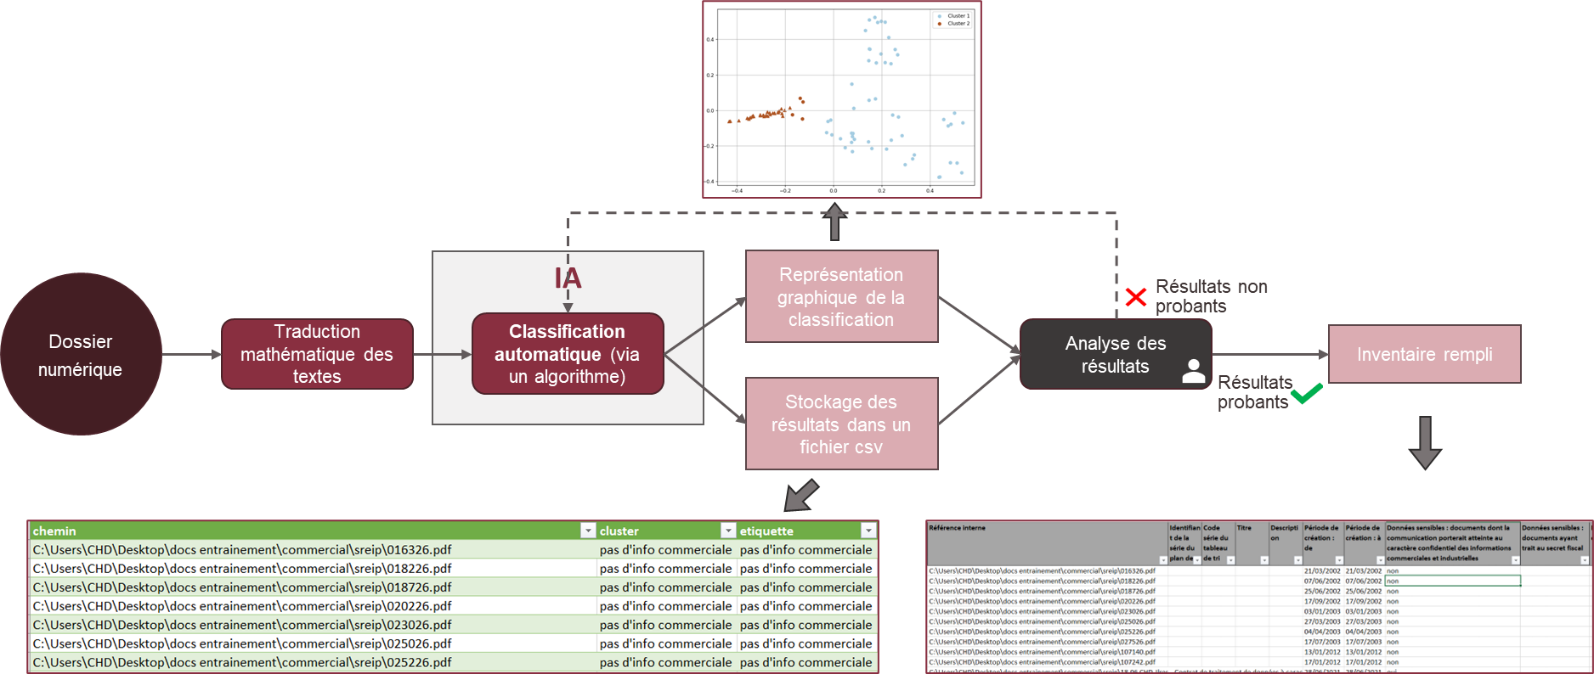
\includegraphics[width=\textwidth]{./media/clustering.png}}
	\caption{Exemple de processus de classification automatique : Clustering sur des documents contenant des informations à caractère commercial}
\end{figure}

Il y a plusieurs méthodes de vectorisation. TF/IDF
consiste à représenter un texte par un vecteur dont les composantes sont
les fréquences des mots dans le document, pondérées par leur importance
dans l\textquotesingle ensemble des documents. Cela met en
évidence les mots qui ont le plus de poids dans chaque document. Nous
avons également défini des \gls{stop-words}, qui sont des mots très
courants dans une langue ou dans le corpus de document, tels que « le »,
« la », « les », etc. qui n\textquotesingle apportent pas
d\textquotesingle information significative pour la classification. En
les éliminant, nous pouvons améliorer la précision de cette dernière.
Notre liste de \gls{stop-words} comportait les mots les plus fréquents
de la langue française et les mots du champs lexical de la législation,
qui se retrouvent dans la plupart des documents. Nous avons également
ignoré les chiffres qui se trouvaient dans les textes. Les vecteurs
obtenus sont des représentations numériques des documents, sous la forme
de tableaux dont chaque valeur correspond à
l\textquotesingle importance d'un mot dans le document.

Une fois ces vecteurs réalisés, il est possible de calculer le texte
le plus proche d'un autre, d'étudier les mots qui ont le plus de
poids pour les ajouter dans les \emph{stop words} s'ils ne sont pas pertinents,
ou d'afficher des groupes de documents les plus proches afin
d'identifier d'éventuels sujets. Après cette étape de vectorisation,
nous avons travaillé sur la classification des documents en appliquant
un algorithme de classification automatique nommé \emph{k-means}. Nous
sommes parvenue, après plusieurs essais, à créer des groupes de
documents à propos d'affaires juridiques et d'ordre commercial
(factures, contrats). Cette méthode était dans une certaine mesure
pertinente pour l'inventaire. Nous étions en mesure de détecter des
documents qui remplissent la colonne «~affaires portées devant des
instances juridictionnelles, extra-judiciaires ou disciplinaires~» et la
colonne «~informations commerciales ou industrielles~». Toutefois, les
textes dans lesquels la mention de ces informations était plus subtile se voyaient
ignorés. Par exemple, un rapport mentionnant de manière implicite une
affaire juridique, sans utiliser de termes spécifiques, passait
inaperçu. Inversement, une loi ou un document issu d'une question
parlementaire sur la justice, donc des documents publics, étaient
détectés comme faisant partie des documents sur des affaires
juridictionnelles. Le multilinguisme pose également problème. Même si la
langue de l'administration parlementaire est le français, le Luxembourg
a trois langues officielles : le luxembourgeois, le français et
l'allemand. De plus, nous avons travaillé sur un fonds relatif aux
relations internationales, ce qui impliquait un certain nombre de
documents en anglais. Il aurait fallu répéter l'ensemble du
processus dans ces quatre langues. Cette méthode n'a donc pas été
choisie pour remplir l'inventaire. Néanmoins, nous en avons retenu les
avantages analytiques des différents tests. Nous avons en effet
expérimenté la méthode avec des nombres différents de \emph{clusters} à
produire par l'algorithme, c'est à dire de groupements de documents
générés automatiquement. Un ensemble de paramètres est modifiable dans
l'algorithme de classification. L'algorithme
\emph{k-means} génère un nombre k
prédéfini de \emph{clusters}, en assignant chaque point au cluster dont il est
le plus proche du centre (centroïde), lui-même déterminé à partir de la
moyenne des coordonnées des points du \emph{cluster}. À chaque itération, nous
tentions de comprendre ce qui liait les documents regroupés. Nous avons
pu en dégager des thèmes, des types de documents et identifier les
différentes langues dans le fonds étudié, puisque les documents se
regroupaient aussi par langue. Ces expérimentations de classification
ont donc constitué une phase productive d'analyse du contenu du fonds.
On pourrait imaginer cette expérimentation comme partie intégrante de la
première étape des pré-traitements de l'archivage numérique, qui
consiste à étudier comment est constitué le fonds, notamment pour
visualiser ce qui est à éliminer. Les techniques de \gls{TAL} sont expérimentées dans 
d'autres projets dans cette même optique analytique. Par exemple, l'application Pêle-mél 
fournit un outil d'analyse des messageries grâce à un système de classification automatique\footcite{noauthor_bilan_nodate}.\newline

D'autres méthodes de classification automatique existent. Plusieurs ont
été testées par des chercheurs indiens sur des jeux de données
d'articles de presse et de critiques de films. Leur objectif était
d'analyser les résultats produits par les différentes méthodes sur des
longs documents\footcite{wagh_comparative_2021}. Dans
cette étude, dix méthodes différentes ont été essayées pour classer
automatiquement des textes longs. Certaines utilisent des modèles de
langage déjà entraînés sur de grandes quantités de texte,
qu\textquotesingle on adapte ensuite à la tâche spécifique de tri des
documents, comme les méthodes \emph{ULMFiT} et \emph{USE (Universal
	Sentence Encoder)}. D\textquotesingle autres s\textquotesingle appuient
sur des réseaux neuronaux, un type de modèle inspiré du cerveau humain,
qui analysent les mots dans l\textquotesingle ordre où ils apparaissent
et utilisent des mécanismes d\textquotesingle attention pour se
concentrer sur les parties les plus importantes du texte. Il y a aussi
des techniques plus classiques, qui comptent la fréquence des mots et
les pondèrent en fonction de leur importance pour le document, comme
\emph{TF/IDF}, que nous avons utilisé, adopté dans l'étude avec l'algorithme de classification \emph{Naive Bayes}. Une
méthode hiérarchique a également été testée, analysant
d\textquotesingle abord les mots, puis les phrases, pour comprendre le
texte dans son ensemble\footcite{wagh_comparative_2021}. Les méthodes de
classification automatique sont donc très diverses. Les résultats de
l'étude montrent que les gros modèles pré-entraînés tendent à offrir de
meilleures performances. Cependant, pour la plupart des jeux de données,
des modèles plus simples\footnote{Ex~: les embeddings de GloVe ou les
	réseaux LSTM peu profonds} peuvent fonctionner avec une perte minimale
en précision.

Les modèles pré-entraînés testés dans le cadre de l'étude sont
\emph{BERT} et \emph{DistilBERT}. Il existe en effet depuis quelques années des moyens
plus précis de vectoriser des documents que les calculs mathématiques de
méthodes comme TF/IDF. Il est possible de réaliser une \gls{vectorisation} qui
aurait une valeur sémantique grâce aux \gls{embeddings}
des grands modèles pré-entrainés tels que les \gls{LLM}). Contrairement à des méthodes comme TF/IDF, ces \emph{embeddings}
capturent la signification contextuelle des mots et rapprochent les
termes ayant des significations similaires dans un même espace
vectoriel. Ces représentations sont générées par des grands modèles de
langage entraînés sur de vastes corpus de textes, ce qui leur permet
d'appréhender des relations complexes entre les mots et
d\textquotesingle offrir une compréhension plus fine et plus nuancée du
contenu sémantique des documents. Ils gèrent également le
multilinguisme lorsqu'ils sont entraînés sur des corpus en plusieurs langues.
Des exemples de modèles d'\emph{embeddings} sont ceux de \emph{BERT},
développé par Google, ainsi que ceux des \gls{LLM} tels
que \emph{GPT-3} et \emph{GPT-4} par \emph{OpenAI}, ou \emph{LlaMa}
\emph{2} par \emph{Meta}. Une autre étude a été réalisée par des
chercheurs et des chercheuses norvégiens pour tester l'efficacité de
différentes méthodes de vectorisation avec de la classification pour
regrouper des articles de presse à propos de mêmes
événements\footcite{tarekegn_large_2024}.
Les meilleures performances étaient obtenues avec des \emph{embeddings} de
\emph{LLM}, puis ceux de \emph{BERT}, suivis par les algorithmes plus
légers et classiques comme \emph{TF/IDF} et \emph{GloVE}\footnote{Technique d'apprentissage automatique pour créer des représentations vectorielles d'entités textuelles en capturant des relations sémantiques entre mots à partir de leurs co-occurrences dans un corpus de texte}
\emph{(Global Vectors for Word Representation)}\footcite{tarekegn_large_2024}.
L'inconvénient principal de ces gros modèles est leur exigence en
puissance de calcul, nécessitant souvent des équipements spécialisés
comme des cartes graphiques (\emph{GPU}). Pour répondre à ce défi, des
versions optimisées des grands modèles de langage ont été développées.
Par exemple, \emph{DistilBERT} est une version allégée de \emph{BERT}
qui est 40 \% plus petite, fonctionnerait 60 \% plus rapidement mais qui
conserverait environ 95 \% des performances du modèle
complet\footcite{noauthor_distilbert_nodate}.
Ce type de modèles n'a pas été testé dans le cadre du projet
\emph{InventAIre}. Nous avons principalement utilisé les grands modèles
de langage pour la génération de texte, sans tester leurs
\emph{embeddings} pour des tâches de classification. Il pourrait être
intéressant de comparer leurs performances avec celles de la méthode
\emph{TF/IDF} sur des documents d'archives pour voir à quel point ils
sont davantage précis. La fourniture de données annotées peut
également améliorer significativement les performances des algorithmes,
il s'agit dans ce cas d'un \gls{supervisé}. Un projet mené par
des chercheurs brésiliens et américains sur la classification
automatique de documents contenant des secrets d'État a par exemple
montré des résultats prometteurs, avec une précision de 90~\% et environ
11~\% de faux positifs\footcite{souza_using_2016}.
Avec de grandes quantités de données, leur méthode pourrait être
applicable au remplissage automatique de l'inventaire des ANLux.
\newline

Une autre perspective réside dans l'extraction de groupes de mots
significatifs à partir de groupements de documents. C'est le concept du
\gls{topic}. Cette méthode permet
d\textquotesingle identifier des thèmes ou sujets sous-jacents dans un
ensemble de textes en regroupant des mots qui apparaissent fréquemment
ensemble. La technique la plus couramment utilisée pour le \emph{topic
	modelling} est \emph{LDA} (\emph{Latent Dirichlet
	Allocation})\footcite{velonis_topic_2022}. 
	\emph{LDA} fonctionne en attribuant chaque document à une
combinaison de sujets et en représentant chaque sujet comme une
distribution de mots. De la même manière qu'avec
l\textquotesingle algorithme \emph{k-means},
l\textquotesingle utilisateur doit définir au préalable le nombre de
groupes, donc le nombre de sujets souhaités. \emph{LDA} distribue alors
les documents et les mots entre ces sujets de manière à maximiser la
cohérence sémantique des groupes formés. Cela permet de dégager les
thèmes principaux abordés dans un corpus de manière automatisée, et sert
ainsi à l\textquotesingle analyse de grands corpus de texte.

Ces méthodes de TAL peuvent fournir des résultats mais nécessitent une série de tests et d\textquotesingle évaluations
pour sélectionner la méthode la plus appropriée, ce qui peut rapidement
devenir déroutant. Pour automatiser une tâche complexe, comme la
rédaction d\textquotesingle un inventaire, avec des ressources limitées,
il est souvent nécessaire d\textquotesingle utiliser une combinaison de
plusieurs méthodes ou modèles. Pour obtenir une bonne précision, il faudra affiner les modèles sur des sous-tâches. Dans le cas du
projet InventAIre, une colonne aurait donc correspondu à un algorithme ou modèle avec des
paramètres qui lui étaient propres.

\subsection{La reconnaissance d'entités nommées}

	Nous avons par ailleurs durant le stage eu l'occasion de tester la
reconnaissance d'entités nommées pour mesurer son efficacité dans la
détection des données à caractère personnel. La reconnaissance d'entités
nommées ou \gls{NER} est une méthode qui
consiste à identifier automatiquement les entités dans un texte. Elles
peuvent être, entre autres, des noms de personnes, de lieux,
d\textquotesingle organisations ou encore des dates. Des bibliothèques
existent en langage Python pour implémenter la reconnaissance d'entités
nommées, telles que \emph{SpaCy} ou \emph{NLTK}, très utilisées dans le
domaine du traitement automatique du langage naturel. Ces bibliothèques
sont basées sur des modèles pré-entraînés capables d'identifier et de
classifier automatiquement les entités dans un texte en analysant le
contexte des mots dans la phrase pour déterminer leur rôle. Elles ont l'avantage d'être gratuites, ouvertes et faciles
d'utilisation. Il est possible d\textquotesingle obtenir rapidement des
résultats avec relativement peu de code. De plus, pour des besoins
spécifiques, il est envisageable de ré-entraîner les modèles de \emph{NER} sur
des corpus personnalisés. Cela améliore la
précision des résultats dans des domaines particuliers ou sur des types
d\textquotesingle entités spécifiques.
Nos expérimentations de \emph{NER} ont suggéré qu'elle était efficace sur la reconnaissance des noms mais malgré ses atouts, elle s'est révélée
insuffisante pour remplir la colonne intitulée «~données à caractère
personnel~» dans l'inventaire. En effet, la loi luxembourgeoise définit
une donnée à caractère personnel comme :

\begin{quote}
	Toute information de quelque nature qu\textquotesingle elle soit et
	indépendamment de son support, y compris le son et
	l\textquotesingle image, concernant une personne identifiée ou
	identifiable (\enquote{personne concernée}); une personne physique ou morale est
	réputée identifiable si elle peut être identifiée, directement ou
	indirectement, notamment par référence à un numéro
	d\textquotesingle identification ou à un ou plusieurs éléments
	spécifiques, propres à son identité physique, physiologique, génétique,
	psychique, culturelle, sociale ou économique\footcite{loi_2002}.
\end{quote}

La définition est donc très vaste et s'étend bien au-delà des noms, des
adresses e-mail ou encore des numéros d'identification personnelle. 

Nous
avons également testé la \emph{NER} dans une perspective de pseudonymisation de
documents. L'objectif était de pseudonymiser des noms dans les titres de
répertoires issus des dossiers RH afin d'être en mesure de sélectionner
des documents que nous pourrions utiliser pour la réalisation de nos
tests d'\gls{apprentissage}. Nous avons développé un script qui
remplaçait automatiquement les noms de personnes, les adresses, les
adresses mail, les noms d'organisations, mais il n'a pas été utilisé. La
définition d'une donnée à caractère personnel illustre bien le fait que
pour pseudonymiser efficacement, il faut détecter et modifier des informations plus subtiles que des
noms, adresses mail, etc. De nombreux outils basés sur des modèles plus complexes ont malgré tout été lancés pour
anonymiser les décisions de justice en Europe. C'est le cas par exemple
à la Cour de Cassation en France dans le cadre d'un projet mentionné
précédemment\footcite{girard-chanudet_travail_2023}.
Ce type de modèle a nécessité une grande quantité de données d'entraînement annotées pour
être performant.
\newline

L'usage principal de la \gls{NER} dans les archives ne concerne pas la
recherche de données personnelles ni la pseudonymisation, mais
l'indexation. C'est un objectif du projet \emph{NER4Archives} porté par les
Archives nationales de France et l'Inria (Institut national de recherche
en sciences et technologies du numérique) débuté en 2020. Ses objectifs
sont la «~conception et réalisation d'un outil de détection, de
classification et de résolution des entités nommées dans les instruments
de recherche archivistiques encodés en XML/EAD\footcite{clavaud_ner4archives_2022}~». 
Le projet part du constat que l'indexation des
inventaires EAD français est souvent insuffisante. Or, une bonne
indexation facilite la recherche dans les archives et la mise en
relation des instruments de recherche. L'architecture de \emph{NER} choisie est
un affinage de celle offerte par la librairie \emph{Spacy}. Cette
dernière utilise \emph{CamemBERT} comme base, un modèle de langage
pré-entraîné basé sur l\textquotesingle architecture \emph{BERT}
mentionnée précédemment, optimisé pour la compréhension et le traitement
du texte en français. Le modèle a par la suite été affiné dans le cadre
du projet sur des instruments de recherche \emph{EAD} annotés. Pour obtenir des
résultats précis en \emph{NER}, il est effectivement souvent nécessaire de
travailler sur des données annotées. Dans le cadre du projet
\emph{NER4Archives}, ce processus d'annotation, qui a duré quatre mois,
a mobilisé quatre annotateurs. Il a permis d'obtenir un \gls{F1-score} 
moyen de 0,91 sur l'architecture la plus performante, en l'occurrence
celle de SpaCy\footcite{clavaud_ner4archives_2022}. Il s'agit d'une bonne performance. Cette précision accrue
grâce aux données annotées est également mise en avant dans le projet
\emph{NewsEye}, dont le but était de produire un je de données multilingue
annoté pour la reconnaissance automatique d'entités nommées\footcite{hamdi_multilingual_2021}.

Dans le processus de traitement de
\emph{NER4Archives}, le processus de \emph{NER} est suivi d'un processus de \gls{NEL}
 pour désambiguïser les entités identifiées et
ainsi éviter les doublons. La \emph{NEL} peut effectivement permettre
d'associer chaque entité à une entrée unique dans un thesaurus ou une
base de données. Au delà des tâches d'indexation, les traitements sur
les entités nommées peuvent offrir la possibilité de nettoyer les
thesaurus. C'est un besoin qui se manifeste à la Chambre des Députés et
dans beaucoup d'administrations. À la Chambre, par exemple, le thesaurus
aurait besoin d'être actualisé. Le personnel chargé de l'indexation des
documents législatifs ajoute régulièrement de nouveaux termes en
fonction des documents traités, mais cela peut entraîner la création de
doublons. Par exemple, le terme «~Covid-19~» a dû être ajouté parce
qu'il était absent du thesaurus. Une autre personne pourrait quant à
elle ajouter «~Covid~» ou «~Coronavirus~», ce qui crée des entrées
équivalentes dans le thésaurus et complique la recherche et
l\textquotesingle organisation des documents.

La reconnaissance d'entités nommées semble être un outil puissant, en
particulier en ce qui concerne l'indexation. En complément de la
classification automatique et du \gls{topic}, la \gls{NER} peut
contribuer à fournir une meilleure description et de meilleurs possibilités
de recherche par entité dans les archives. Ces outils techniques ont
également du potentiel en termes d'évaluation de gros corpus pour
détecter des documents à éliminer. La \emph{NER} est par exemple intégrée au
logiciel de traitement des mails \emph{ePADD} en partie dans cette optique de
tri\footcite{lee_computer-assisted_2018}. Malgré leur
complexité, ces méthodes
offrent une approche analytique approfondie des fonds.

\subsection{Le traitement automatique sur les images}

Le dernier type de traitement automatique via des algorithmes plus
légers que les grands modèles de langage est le traitement des images.
La pratique de la reconnaissance automatique de caractères est l'usage
du \emph{machine learning} le plus répandu dans les services d'archives, parce
qu'elle nécessite peu de connaissances techniques, étant intégrée à de
nombreux logiciels. Les Archives nationales du Luxembourg et la BNL travaillent par exemple
sur des projets d'\gls{HTR} à l'aide du logiciel \emph{Transkribus}.
Nous avons intégré une étape d'\gls{OCR} à notre traitement de données pour générer l'inventaire.
A chaque nouveau document traité, si le texte n'est pas disponible, l'outil développé tente de l'extraire.
Pour cela, nous transformons le document en image dans notre environnement Python, avant d'utiliser la
librairie \emph{Tesseract} pour en extraire le texte. Ce traitement excluait les documents contenant des écritures manuscrites, 
qui sont loin d'être majoritaires dans les vracs bureautiques, mais on pourrait imaginer la reconnaissance automatique sur ces fichiers dans le futur
si le projet continue.

Nous n'avons pas réalisé d'autres traitements sur les images dans le
cadre du projet InventAIre, mais nous y avons réfléchi. Nous avons par
exemple émis l'hypothèse que les actes notariés pourraient être
reconnus automatiquement grâce à la présence d'un tampon de notaire, de
même pour les actes d'état civil. Un modèle de détection de tampons a
été mis en place par un groupe de chercheurs. Il fonctionne avec l'algorithme de détection d'objets \emph{YOLO (You Only
Look Once)} comme base. Ce modèle est décrit comme «~efficace, contenant
un petit nombre de paramètres et {[}pouvant{]} être exécuté rapidement
sur des appareils mobiles\footcite{gayer_fast_2022}~»[Traduction libre]. Les modèles basés sur
l'analyse d'image sont en effet moins volumineux que les modèles de
traitement automatique du langage car ils opèrent sur des pixels, donc des données en deux dimensions minimum (pixel
noir ou blanc). Des filtres peuvent permettre de réduire le nombre de
dimensions en cas de traitement d'images en couleur. Les modèles de TAL
doivent quant à eux modéliser des relations complexes dans des séquences
de texte, et possèdent donc bien plus de paramètres. Nous aurions pu
imaginer le développement d'un modèle détectant les tampons liés à l'État
civil ou de notaires, qui, pour être plus précis, aurait été
associé à du TAL. Ces modèles qui mélangent les deux types de traitement
sont des modèles multimodaux. Des chercheurs ont travaillé sur ce type
d'outils pour la classification de documents d'archives turques, développant
 un algorithme de classification qui classifie à la fois les
images et le contenu textuel après océrisation\footcite{durukan_multimodal_2024}. La précision de
l'algorithme serait supérieure à 96~\%\footcite{durukan_multimodal_2024}, ce qui est prometteur.

Le traitement des images et la détection d'objets sont par ailleurs utiles
à l'indexation des documents graphiques. Un projet a été lancé sur
l'indexation des photos du gouvernement par le Service information et
presse du gouvernement du Luxembourg dans le cadre de l'initiative
\emph{AI4Gov} mais nous avons trouvé peu d'informations sur ce
dernier\footcite{noauthor_initiative_2021}.
Ce type de projets se multiplie dans le monde des bibliothèques et des
archives. En France, le prototype de \emph{GallicaPix} a été lancé en
2021. Basé sur la détection d'objets, il sert à effectuer des recherches par contenu iconographique dans les contenus de la BnF.
Ce genre de projets pourrait être aussi mené dans les archives pour indexer des images par contenu par exemple.
L'intelligence artificielle pour le traitement des images a été exploitée dans le domaine de l'\gls{OCR} et de l'\gls{HTR}, mais 
reste encore à explorer pleinement, notamment pour l'indexation automatique de contenu audiovisuel.

\subsection{Des usages sur les tâches aux impacts moins	élevés~: recherche, indexation et \gls{découvrabilité}}

Comme nous l'avons vu, de nombreuses méthodes de traitement automatique
peuvent être appliquées sur des fonds numérisés ou nativement
numériques. Elles ont chacune leurs avantages et leurs inconvénients. La
classification automatique et le \emph{topic modelling} sont par exemple
complexes à appréhender techniquement. Ils reposent sur des logiques
mathématiques dont il faut être en mesure de comprendre les bases. Des
précautions sont par exemple à prendre au moment d'appréhender les
graphiques représentant des résultats de classification automatique. Les vecteurs
peuvent être des vecteurs de plusieurs milliers de dimensions, or, ils sont
réduits à deux dimensions pour être représentés sur un graphique. Des
métriques sont par conséquent à calculer pour vérifier la qualité de la
réduction de dimension, pour s'assurer que les groupes formés sont
réellement aussi groupés qu'ils ne l'apparaissent sur le graphique. Un autre inconvénient de
la classification est le fait que les petits groupes sont plus
difficiles à identifier par la machine. Un certain bagage technique ou
des recherches sont nécessaires avant de prendre en main ce genre
d'algorithmes et des précautions sont à prendre avant de diffuser des
graphiques de classification. Les limites sont également d'ordre
matériel~: les besoins en termes de puissance de calcul augmentent plus
les modèles sont gros et plus les corpus à traiter sont grands. On peut
s'interroger sur la nécessité d'utiliser les \emph{embeddings} de gros
modèles pré-entraînés pour la classification si l'objectif est
analytique. En effet, des groupes se dégagent avec des méthodes
classiques. Dans le cadre du projet \emph{InventAIre}, la méthode
\emph{TF/IDF} a permis d'identifier des groupes pertinents et de mieux
appréhender le contenu du fonds à traiter. Sur le plan analytique, une
meilleure précision dans les groupes n'aurait peut-être pas eu un grand
impact. Il s'agit potentiellement d'une piste à explorer. 

La classification automatique présente par ailleurs l'avantage d'être une
méthode rapide à coder. La partie code de la
classification nous a demandé deux heures tout au plus.
Le plus long est de tester avec différents paramètres, d'examiner les
différents groupes à chaque itération et de créer des sauvegardes quand
les résultats sont pertinents. Il faut tâtonner pour obtenir des
résultats. Cet aspect a été souligné par Seth van Hooland et Mathias Coeckelbergs 
dans un article explorant les possibilités et limites du \emph{topic modelling} et du \emph{word embedding}. Ils évoquent que les paramètres et les termes inclus en tant que \gls{stop-words} ont un
impact non négligeable sur les résultats\footcite{van_hooland_unsupervised_2018}. Ils parlent du caractère «~boîte noire~» de ces
méthodes\footcite{van_hooland_unsupervised_2018} et concluent en disant que l'application
des techniques d'apprentissage automatique présente une «~nature
semi-automatisée~» et qu'«~à des étapes cruciales du processus, les
experts en archivistique doivent encore prendre des décisions
stratégiques et intervenir manuellement~»\footcite{van_hooland_unsupervised_2018}[Traduction libre]. Il en va
de même pour le \emph{topic modeling} : les «~résultats [sont] satisfaisants mais obscurs\footcite{meeks}~»[Traduction libre]. Les
limites et les avantages sont similaires à ceux de la classification.
Les deux servent au \emph{disant reading}\footcite{meeks}, c'est à dire
à découvrir des motifs ou des tendances dans des grands corpus sans
avoir à les explorer dans leur intégralité, mais la production de
résultats satisfaisants demande des expérimentations et un grand travail
d'analyse.\newline

Les perspectives archivistiques des modèles de \gls{NER}, de \gls{NEL} et de la
classification automatique sont diverses. Néanmoins, comme évoqué en
première partie, il est important de définir des cas d'usage pertinents
pour ces technologies, de s'interroger sur la nature des usages qui
offrent le meilleur équilibre entre facilité de mise en production et
valeur ajoutée. Comme nous avons pu le voir, la classification automatique et le \emph{topic
	modelling} ne sont pas une solution miracle pour automatiser un
traitement aussi complexe que le classement d'unités de description dans
l'inventaire des ANLux. Ils sont utiles néanmoins pour visualiser les
documents similaires dans les archives, identifier les mots
significatifs et ainsi différents sujets dans le corpus, et constituent
des outils d'analyse de ce dernier dans sa globalité. Ils peuvent être
également intéressants dans une optique de \gls{découvrabilité},
par exemple par la proposition du document le plus proche d'un autre
dans l'espace vectoriel à un lecteur. Cet usage a un impact moins
important en cas d'erreur que des données sensibles non repérées. 

Ces
techniques peuvent également servir à la recherche, en produisant des
\emph{dashboards} de visualisation de documents ou de groupements
thématiques. Il en va de même pour le traitement automatique des images, qui
permet une meilleure indexation et description de leur contenu, mais qui
nécessite plus de recherches et de développement avant d'être efficace
sur l'automatisation de tâches archivistiques complexes. La question de
la découvrabilité et de l'efficacité des outils de recherche n'est pas
prioritaire au Luxembourg mais demeure un défi archivistique. De même, en
France, la question se pose dans les bibliothèques, mais concernant les
Archives nationales, Bruno Ricard a rappelé lors de la Journée des
archivistes luxembourgeois le 7 juin 2024, que la priorité était de bâtir
un système d'information archivistique solide, avant de se pencher plus
précisément sur ce sujet et celui de l'intelligence artificielle. Il est
cependant possible de s'interroger sur le fait qu'une excellente
découvrabilité et des moteurs de recherche efficaces puissent compenser
une description archivistique insuffisante.\newline

D\textquotesingle un point de vue technique, les limites matérielles et intellectuelles se manifestent rapidement en ce qui concerne le \gls{TAL} et la
classification d'images. Comme mentionné précédemment, il est souvent
nécessaire de diviser les grandes tâches en sous-tâches plus
spécifiques, chacune étant traitée par un modèle distinct. Bien que
l\textquotesingle utilisation d\textquotesingle algorithmes légers
permette d'automatiser, ou au moins de gagner du temps sur certaines
tâches, elle complexifie la \gls{chaîne} des archives. Il serait
donc pertinent de mesurer l'efficacité de cette approche par rapport à
l'utilisation de modèles plus généraux, comme les \gls{LLM}, plus volumineux mais potentiellement plus efficaces et
générant moins de complexités dans la chaîne de traitement.


